\documentclass[11pt,letterpaper]{article}
\usepackage[utf8]{inputenc}
\usepackage[spanish]{babel}\decimalpoint
\usepackage{amsmath}
\usepackage{amsfonts}
\usepackage{amssymb}
\usepackage{physics}
\usepackage{hyperref}
\usepackage[left=2cm,right=2cm,top=2cm,bottom=2cm]{geometry}


\usepackage{graphicx}
%\graphicspath{{img_tarea07/}}
\usepackage{subfigure}
\usepackage{caption}
\usepackage{dsfont}


\usepackage[draft,inline,nomargin]{fixme} \fxsetup{theme=color}
\definecolor{jacolor}{RGB}{200,40,0} \FXRegisterAuthor{ja}{aja}{\color{jacolor}JA}

\newcommand{\mcM}{\mathcal{M}}
\newcommand{\id}{\mathds{1}}

\renewcommand{\labelenumii}{\arabic{enumi}.\arabic{enumii}}
\renewcommand{\labelenumiii}{\arabic{enumi}.\arabic{enumii}.\arabic{enumiii}}
\renewcommand{\labelenumiv}{\arabic{enumi}.\arabic{enumii}.\arabic{enumiii}.\arabic{enumiv}}

%%%%% Author
\author{José Alfredo de León}

%%%% Title 
\title{Tarea 7\\
\large{Métodos de Simulación Computacional para Sistemas Cuánticos - 2022-2}}


\begin{document}
\date{25 de abril de 2022}
\maketitle

\section{Objetivos}
\subsection{Objetivo general}
Construir el diagrama de fase del modelo de Bose-Hubbard numéricamente
utilizando un algoritmo auto-consistente y analíticamente utilizando
teoría de perturbaciones.

\subsection{Objetivos específicos}
\begin{enumerate}
\item Utilizar la aproximación de desacoplamiento en el modelo de Bose-Hubbard.
\item Implementar el algoritmo auto-consistente para encontrar numéricamente
el diagrama de fases del modelo de Bose-Hubbard.
\item Reproducir el mismo diagrama de fase con el algoritmo auto-consistente 
y con la expresión analítica obtenida con teoría de perturbaciones.
\item Determinar el comportamiento de la fluctuación de partículas en 
el estado fundamental del modelo de Bose-Hubbard.
\item Revisar el comportamiento de convergencia del algoritmo auto-consistente.
\end{enumerate}

\section{Marco teórico}
En la aproximación de desacoplamiento 
$\qty(b_i^{\dagger}-\expval{b_i^{\dagger}})\qty(b_j-\expval{b_j})\approx 0$
podemos escribir al Hamiltoniano efectivo por sitio del modelo de Bose-Hubbard, suponiendo 
que el sistema es homogéneo y con invarianza traslacional, como
\begin{align}\label{eq:BH:Hamiltonian}
H=-\sigma \psi \qty(\hat b+\hat b^{\dagger})+\sigma \psi^2+
\frac{1}{2}U\hat n\qty(\hat n-\id)-\mu \hat n,
\end{align}
donde hemos denotado $\sigma=zt$, con $z$ el número de vecinos próximos y 
$t$ el parámetro de \textit{hopping}. Se utiliza esta notación para ser 
consistentes con las variables utilizadas en la implementación.
Además, $\psi$ es el parámetro de orden de la fase superfluída,
$U$ el parámetro de interacción y $\mu$ el potencial químico. Los
operadores de creación $\hat b^{\dagger}$, aniquilación $\hat b$ 
y el operador de número $\hat n$ se escriben en su representación matricial 
como
\begin{align}
b&=\mqty(0&\sqrt{1}&0&\cdots&0\\
0&0&\sqrt{2}&\ddots&\vdots\\
0&0&0&\ddots&0\\
\vdots&\vdots&\vdots&\ddots&\sqrt{N}\\
0&0&0&\cdots&0) &
b^{\dagger}&=\mqty(
0&0&0&\cdots&0\\
\sqrt{1}&0&0&\cdots&0\\
0&\sqrt{2}&0&\cdots&0\\
\vdots&\ddots&\ddots&\ddots&\vdots\\
0&\cdots&0&\sqrt{N}&0) &
n=\mqty(
\sqrt{1}&0&0&\cdots&0\\
0&\sqrt{2}&0&\cdots&0\\
0&0&\sqrt{3}&\ddots&0\\
\vdots&\vdots&\vdots&\ddots&0&\\
0&0&0&0&\sqrt{N}
), 
\end{align}
donde $N$ es la dimensión de cada sitio en la red unidimensional.

De forma usual, la fluctuación de partículas por sitio se escribe
\begin{align}
(\Delta n)^2=\expval{\hat n^2}-\expval{\hat n}^2.
\end{align}

La ventaja numérica que supone el Hamiltoniano del modelo de Bose-Hubbard
en la aproximación de desacoplamiento es que su representación matricial 
es tridiagonal, lo cuál hace viable resolver el problema de construir 
numéricamente el diagrama de fase para determinar la fase superfluída
($\psi\neq 0$) y la fase de aislante de Mott ($\psi=0$), así como la región
de transición entre fases.

Por otro lado, utilizando teoría de perturbaciones independiente del tiempo 
no degenerada uno puede encontrar, a segundo orden, la energía del 
estado base y así encontrar la condición para que ocurra una 
transición de fase cuántica, siendo esta condición la siguiente:
\begin{align}
y=\frac{-\tilde g^2+2x\tilde g+\tilde g-x^2-x}{1-x},
\end{align}
con $y=\sigma /U$ y $x=\mu / U$. 

Además, de esta expresión podemos inferir una expresión para 
el potencial químico:
\begin{align}
\frac{\mu}{\sigma}=\frac{1}{2}\frac{U}{\sigma}\qty(2g-1)-1\pm
\frac{1}{2}\pm \sqrt{\qty(\frac{U}{\sigma})^2-2\frac{U}{\sigma}\qty(2g+1)+1}.
\end{align}


\section{Qué se hizo}\label{sec:queHacer}
En este trabajo se realizó el diagrama de fase típico
del modelo de Bose-Hubbard donde se observan las fases cuánticas de 
aislante de Mott y superfluída. Por un lado, se implementó un algoritmo
autonconsistente para encontrar el parámetro de orden superfluído $\psi^2$ y,
por otro lado, se utilizaron las expresiones analíticas de la teoría de 
perturbaciones (ecuaciones 4 y 5). Dada las diferentes formas de presentar el diagrama de fase 
en materia condensada y en física atómica se realizaron los diagramas de 
fase escalando al potencial químico con la energía de interación $U$ y 
la interacción entre sitios $zt$, respectivamente. Adicionalmente, 
se calculó numéricamente la fluctuación de partículas del estado fundamental.
También se llevó cuenta de la cantidad de pasos que le toma al algoritmo 
autoconsistente en converger considerando una tolerancia de error de 
$10^{-6}$.


\section{Implementación}
A continuación, describimos el algoritmo auto-consistente.

\textbf{Entrada}: valores de $\mu$, $U$ y $\sigma$ ($zt$). 
\textbf{Salida}: parámetro de superfluído
$\psi$, estado base $\ket{\psi_G}$ y número de pasos antes de el 
algoritmo converja.
\textbf{Necesita}: rutinas \texttt{H[]} y \texttt{GroundState[]},
que implementan, respectivamente, al Hamiltoniano de la ecuación 
\eqref{eq:BH:Hamiltonian} y el eigensolver para encontrar la eigenenergía y 
el eigenvector del estado fundamental.
\begin{enumerate}
\item Establecer $\psi=\psi_0=0.1$
\item Evaluar $H(\psi_0)$
\item Obtener el estado base de $H(\psi_0)$
\item Calcular el valor esperado del operador de aniquilación
y asignar el nuevo valor $\psi=\matrixel{\psi_g}{\hat b}{\psi_g}$
\item Calcular $\text{error}=\abs{\psi-\psi_0}$
\item Establecer $\psi_0=\psi$ y repetir desde el paso 2 hasta que \textbf{ya
no} se satisfaga la condición $\text{error}>10^{-6}$.
\end{enumerate}


\section{Resultados y discusión}
\subsection{Resultados}
En las gráficas de las Figs. 1, 2 y 3 se muestras, respectivamente, 
el diagrama de fase del modelo de Bose-Hubbard, fluctuaciones de partículas
en el estado fundamental y número de pasos que le tomó para converger 
al algoritmo auto-consistente para calcular el parámetro de orden 
superfluído $\psi ^2$.
\begin{figure}
\centering
\subfigure[]{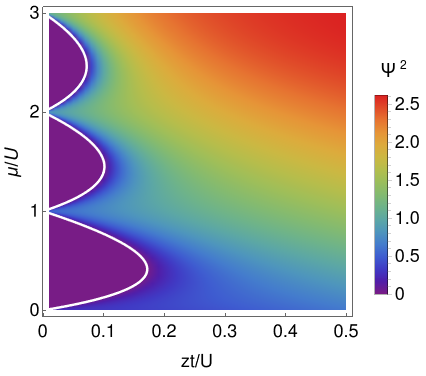
\includegraphics[width=8.5cm]{img_tarea07/fraccion_condensado_01.png}}
\subfigure[]{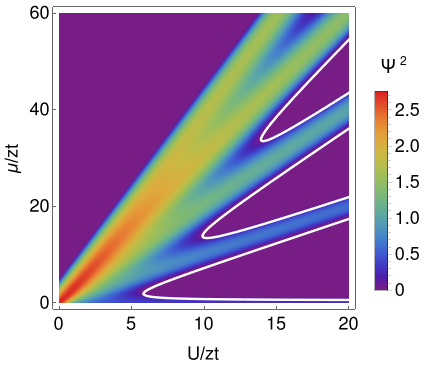
\includegraphics[width=8.5cm]{img_tarea07/fraccion_condensado_02.png}}
\caption{Diagrama de fase del modelo de Bose-Hubbard. (a) Presentación
de materia condensada. (b) Presentación de Física Atómica.}
\end{figure}

\begin{figure}[t]
\centering
\subfigure[]{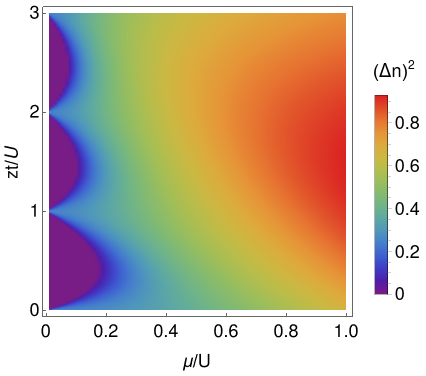
\includegraphics[width=8.5cm]{img_tarea07/fluctuacion_particulas_01.png}}
\subfigure[]{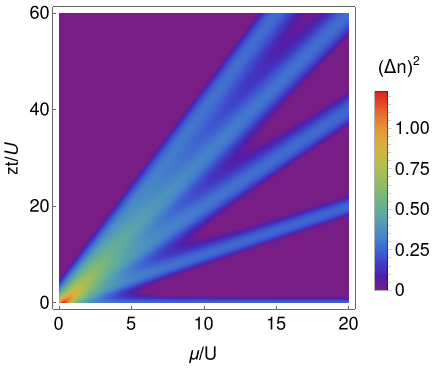
\includegraphics[width=8.5cm]{img_tarea07/fluctuacion_particulas_02.png}}
\caption{Fluctuación de partículas del modelo de Bose-Hubbard en el estado
fundamental. (a) Presentación de materia condensada. (b) Presentación de
Física Atómica.}
\end{figure}

\begin{figure}
\centering
\subfigure[]{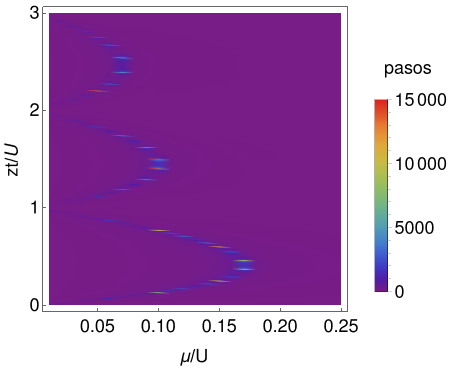
\includegraphics[width=8.5cm]{img_tarea07/pasos_01.png}}
\subfigure[]{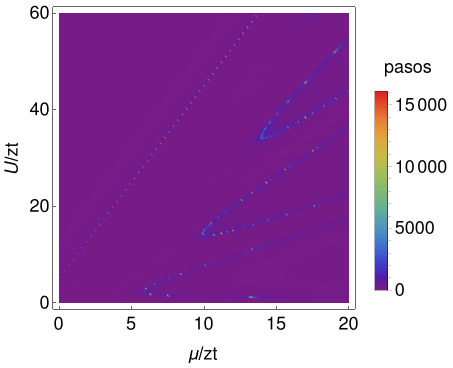
\includegraphics[width=8.5cm]{img_tarea07/pasos_02.png}}
\caption{Cantidad de pasos que le tomó al algoritmo auto-consistente
converger en función de los mismos parámetros que se hicieron variar 
en el Hamiltoniano para constuir el diagrama de fase del modelo de
Bose-Hubbard.}
\end{figure}


\subsection{Discusión y conclusiones}
Se consiguió exitosamente reproducir el diagrama de fase del 
modelo de Bose-Hubbard expuesto en la Fig. 4 de \cite{caballero2022materia}.
Según la presentación que prefiramos, vemos en la Fig. 1 que hay diferentes
regiones que representan la fase de aislante de Mott, mostrando 3 regiones 
en nuestros resultados, mientras la fase superfluída ``envuelve'' a las
regiones de aislante de Mott. Estas regiones de aislante de Mott se pueden
distinguir de mejor manera si observamos las curvas blancas que las delimitan,
calculadas con teoría de perturbaciones. 

Respecto a la fluctuación de partículas por sitio, vemos en la Fig. 2 que
dentro de las regiones de aislante de Mott no existe fluctuación de partículas;
esta sólo ocurre en la fase superfluída, aumentando conforme aumenta el
potencial químico y disminuye la energía de interacción.

Por último vamos a comentar sobre el comportamiento del algoritmo auto-consistente
para calcular el parámetro de orden superfluído. En la Fig. 3 nuestras 
gráficas muestran que la cantidad de pasos para converger es mucho mayor 
a cero únicamente en la región de transición entre las dos fases cuánticas
del modelo de Bose-Hubbard. Fuera de la ``frontera'' de transición
entre fases el algoritmo converge con una cantidad de pasos cercana a cero.


\bibliographystyle{unsrt}
\bibliography{references}

\end{document}